%----------------------------------------------------------------------------------------
%	PACKAGES AND OTHER DOCUMENT CONFIGURATIONS
%----------------------------------------------------------------------------------------

\documentclass[12pt,a4paper,twoside]{book}
\usepackage{times}
\usepackage[latin1]{inputenc}
\usepackage[italian]{babel}
\usepackage{amsmath}
\usepackage{amsfonts}
\usepackage{amssymb}
\usepackage{graphicx}
\usepackage{setspace}
\usepackage{fancyhdr}
\usepackage{emptypage}
\renewcommand{\baselinestretch}{1.5} 
%sommario
%profondit� 1 = sezioni (2 = sottosezioni ecc..)
\setcounter{tocdepth}{1}
\onehalfspacing
%numeri di pagina dispari a dx e pari a sx nel pi� di pagina
\pagestyle{fancy}
\fancyhf{}
\fancyfoot[LE,RO]{\thepage}
\fancypagestyle{plain}{\fancyfoot[RO,LE]{\thepage}}


%----------------------------------------------------------------------------------------
%	TITLE SECTION
%----------------------------------------------------------------------------------------

\author{Fabio Terzi, Matteo Zambelli} % Your name

\begin{document}
	
\tableofcontents % l'indice


%----------------------------------------------------------------------------------------
%	introduzione
%----------------------------------------------------------------------------------------

\chapter{Introduzione}

Il progetto 3D4Amb mira a sviluppare un sistema basato sul 3D per la diagnosi e il trattamento dell?ambliopia nei bambini piccoli.\\
Sfrutta la tecnologia 3D active shutter per garantire una visione binoculare, cio� per mostrare immagini diverse all'occhio normale e all'occhio pigro. Essa dovrebbe consentire una facile diagnosi dell'ambliopia e il suo trattamento per mezzo di giochi interattivi e attivit� di intrattenimento. Non dovrebbe soffrire dei problemi del trattamento classico dell'occlusione, � adatto ad un uso domestico, e potrebbe, almeno in parte, sostituire l'occlusione dell'occhio normale.\\                           
L'obiettivo principale di questo progetto di ricerca, denominato 3D4Amb, � di sviluppare un sistema per la diagnosi e il trattamento di ambliopia, basata sulla visione binoculare in modo accessibile. Con il termine accessibile si intende: poco costoso, user friendly, adatto per uso domestico e facilmente estendibile.\\
Tutte le informazioni sul progetto sono reperibili sul sito: http://3d4amb.unibg.it/
Car Racing Cardboard � un'applicazine per la piattaforma Android, il suo scopo � curare una patologia come l?ambliopia attraverso un gioco, in modo tale da far divertire il paziente ed allo stesso tempo sottoporlo al trattamento per la cura della sua malattia.

%----------------------------------------------------------------------------------------
%	l'ambliopia
%----------------------------------------------------------------------------------------

\chapter{L'Ambliopia}

\section{Il disturbo}
L'ambliopia � una condizione di ridotta acuit� visiva mono o bilaterale e si manifesta indipendentemente da causa organica. � dovuta ad una inadeguata stimolazione visiva
durante il periodo plastico del sistema visivo, ossia il periodo che va dalla nascita fino ai sette anni.\\
Il soggetto in cui � presente l'ambliopia soffre di un alterazione della visione dello spazio: le immagini che provengono dagli occhi non vengono correttamente rielaborate all'interno del cervello. Questo causa una scorretta comprensione dello spazio che lo circonda e causa una percezione scorretta della profondit�, dei movimenti e dei contrasti.
� presente nel 2-4\% della popolazione, la sua incidenza � pi� elevata in associazione con alcune condizioni quali prematurit�, sindrome di Down, patologia neurologica e familiarit� per ambliopia o strabismo. Spesso le persone non si accorgono nemmeno di esserne affette fino ai 20-30 anni, per questo � fondamentale la diagnosi.\\
Pu� colpire i bambini dalla nascita fino ai 7 anni, et� in cui il sistema visivo raggiunge la sua maturit�. Durante questo periodo iniziale l?ambliopia pu� essere trattata e prevenuta, mentre superata questa fase l?istaurazione della malattia diventa impossibile, ma, nel caso fosse presente, essa risulta irreversibile. L?ambliopia funzionale deve essere distinta dall?ambliopia organica, la quale � un impoverimento della visione, causata da anomalie strutturali dell?occhio o del cervello, che sono indipendenti dagli input sensoriali.\\
L'ambliopia funzionale � reversibile se trattata con la stimolazione visiva adeguata, mentre quella organica non subisce alcun beneficio da una stimolazione visiva.
Il videogame di rebalance ha quindi effetto solo sull' ambliopia funzionale e non su quella organica.

\section{Trattamenti}
Il trattamento precoce dell?ambliopia � fondamentale per ottenere buoni risultati, la correzione oculare avviene in diversi modi:

\subsection{Occlusione}
La terapia occlusiva si basa sulla copertura dell?occhio sano per stimolare l?occhio ambliope. Solitamente nei pazienti affetti anche da strabismo l?occlusione avviene a tempo pieno; tuttavia l?occlusione  a tempo pieno, o occlusione totale, pu� causare un ambliopia inversa nei soggetti sotto i 4-5 anni. Per evitare l?insorgere di questo ulteriore problema, la condizione dell? ambliopia deve essere monitorata ogni settimana per l?et� del bambino. Per esempio, un bambino di due anni va monitorato ogni due settimane, uno di tre ogni tre settimane. Nel caso in cui venga riscontrato che il paziente non sopporta un?occlusione totale si applica un? occlusione parziale, ossia solo qualche ora al giorno.

\subsection{Penalizzazione ottica}
Attuata con filtri di Bangerter (lenti con gradi diversi di opacizzazione, a seconda della entit� della penalizzazione che si vuole attuare) o con  lenti pi� forti o pi� deboli poste davanti all'occhio sano per costringere quello malato a lavorare; come l'occlusione parziale, viene attuata o per coloro che  necessitano di una occlusione "morbida" o come terapia di mantenimento.

\subsection{Penalizzazione farmacologica}
Viene effettuata con un collirio cicloplegico instillato nell?occhio sano per escluderlo dal processo di visione e  costringere quello malato a lavorare.

\subsection{Settorizzazione}
Consiste nella copertura di parte del campo visivo dell?occhio sano con pellicole adesive traslucide sugli occhiali. \\
Per il trattamento dell'ambliopia sono stati proposti anche degli stimolatori visivi di tipo elettrico (trattamento CAM-Cambridge Stimulator e trattamento Flicker): vengono inviati stimoli luminosi di vario tipo sulla retina dell'occhio ambliope, forzandolo  a trasmettere l'impulso luminoso al cervello, e riattivando cos� i canali "impigriti" dall'ambliopia. L'efficacia di queste metodiche � ancora oggi molto dibattuta.  Recentemente si stanno utilizzando farmaci neuroprotettivi come sostegno alla terapia occlusiva: studi recenti indicano che in questo modo viene potenziato l'effetto della terapia occlusiva e viene pi� facilmente stabilizzato il miglioramento della funzione visiva.

\section{L'idea di 3D4Amb}
3D4Amb ha ideato un sistema basato sulle tecnologie 3D per consentire la visione binoculare. L'uso classico di un sistema 3D � quello di fornire ai due occhi diverse immagini della stessa scena con angoli di visualizzazione leggermente sfalsati che corrispondono ai diversi punti di vista dell? occhio destro e sinistro. Questa visione produce un'illusione di profondit� della scena ed � la base della realt� virtuale.\\                                                         
Il principio primario del sistema � che all?occhio ambliope (o occhio pigro) e all'occhio normale sono mostrate due immagini differenti ma correlate. Questo principio pu� essere utilizzato nella pratica per il trattamento di ambliopia, andando a mostrare all'occhio ambliope la parte pi� interessante dei frame della clip o del gioco, mentre all'occhio non ambliope (o buono) viene mostrata la parte meno interessante.\\
Il contenuto da mostrare al paziente (gioco o immagine) viene diviso da 3D4Amb in due parti, una per l'occhio destro (occhio ambliope, Figura ~\ref{idea 3D4Amb}) e una per l'occhio sinistro (occhio buono, Figura ~\ref{idea 3D4Amb}). Il software 3D4Amb decider� cosa inviare ad entrambi gli occhi a seconda del tipo di trattamento suggerito dal medico. Si noti che l'occhio pigro del bambino � pi� stimolato a lavorare, ma l'occhio sano non � ?patchato?. Il cervello del paziente ha il compito di unire le due immagini per visualizzare il frame completo con successo ed eseguire correttamente operazioni semplici in caso di gioco interattivo. Per assicurarsi che il paziente possa unire le due immagini sono presenti un numero significativo di elementi comuni ad entrambe le immagini. Notare che il frame finale � una rappresentazione bidimensionale in quanto l'obiettivo � quello di non stimolare la visione stereo del paziente (almeno inizialmente).\cite{tesiTZ}

\begin{figure}[t]
	\centering
	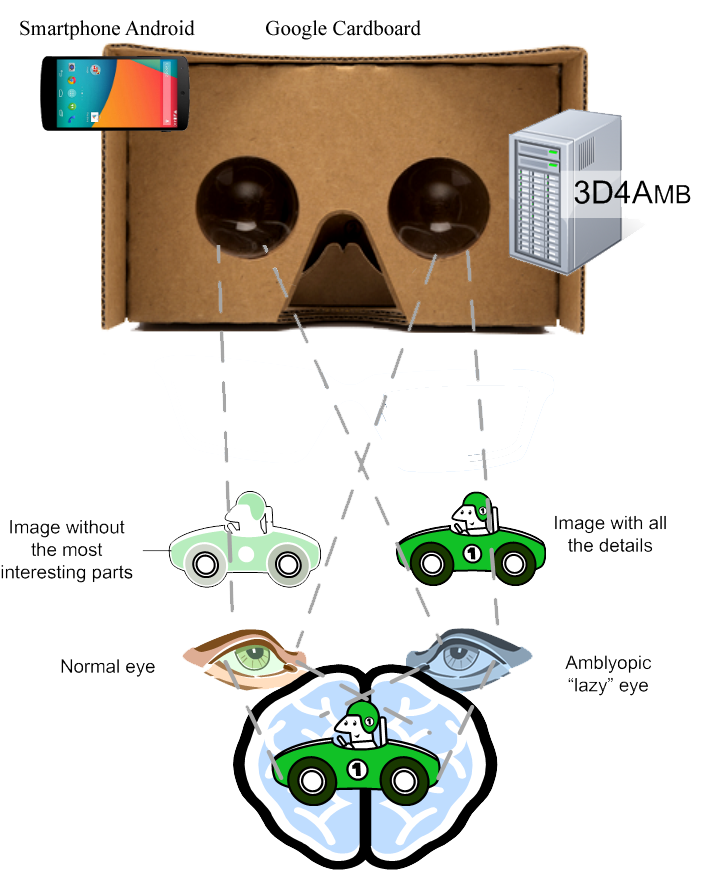
\includegraphics[width=\columnwidth]{immagini/3D4Amb_sys.png}
	\caption{La tecnologia di 3D4Amb \label{idea 3D4Amb}}
\end{figure}



%----------------------------------------------------------------------------------------
%	il prinicipio del trattamento
%----------------------------------------------------------------------------------------

\chapter{Il principio del trattamento tramite il gioco}

%----------------------------------------------------------------------------------------
%	l'applicazione
%----------------------------------------------------------------------------------------

\chapter{Car racing cardboard: l'applicazione}

%----------------------------------------------------------------------------------------
%	raccolta dati
%----------------------------------------------------------------------------------------

\chapter{??Raccolta dati??}

%----------------------------------------------------------------------------------------
%	social media
%----------------------------------------------------------------------------------------

\chapter{Social media}

%----------------------------------------------------------------------------------------
%	paper
%----------------------------------------------------------------------------------------

\chapter{Paper}

%----------------------------------------------------------------------------------------
%   conclusioni
%----------------------------------------------------------------------------------------

\chapter{Conclusioni}

%bibliografia
\bibliography{tesi} 

\end{document}